% Run in this directory: pdflatex -jobname=fig_bon_bridge_bootstrap fig_bon_bridge_bootstrap_labels.tex
% Clean labels: pdflatex -jobname=fig_bon_bridge_bootstrap_clean '\def\cleanreview{1}% Run in this directory: pdflatex -jobname=fig_bon_bridge_bootstrap fig_bon_bridge_bootstrap_labels.tex
% Clean labels: pdflatex -jobname=fig_bon_bridge_bootstrap_clean '\def\cleanreview{1}% Run in this directory: pdflatex -jobname=fig_bon_bridge_bootstrap fig_bon_bridge_bootstrap_labels.tex
% Clean labels: pdflatex -jobname=fig_bon_bridge_bootstrap_clean '\def\cleanreview{1}% Run in this directory: pdflatex -jobname=fig_bon_bridge_bootstrap fig_bon_bridge_bootstrap_labels.tex
% Clean labels: pdflatex -jobname=fig_bon_bridge_bootstrap_clean '\def\cleanreview{1}\input{fig_bon_bridge_bootstrap_labels.tex}'
% The original PDF is embedded unchanged. Only label areas are covered.
\documentclass[tikz,border=0pt]{standalone}
\usepackage[OT1]{fontenc}
\usepackage{amsmath,graphicx,xcolor}
\newcommand{\labelchange}[2]{%
  \ifdefined\cleanreview #1\else\textcolor{red}{#1}\\\textcolor{blue}{(#2)}\fi}
\begin{document}
\begin{tikzpicture}[x=1bp,y=-1bp,every node/.style={inner sep=0pt,align=center,font=\sffamily\fontsize{5}{5.5}\selectfont}]
\node[anchor=north west] at (0,0) {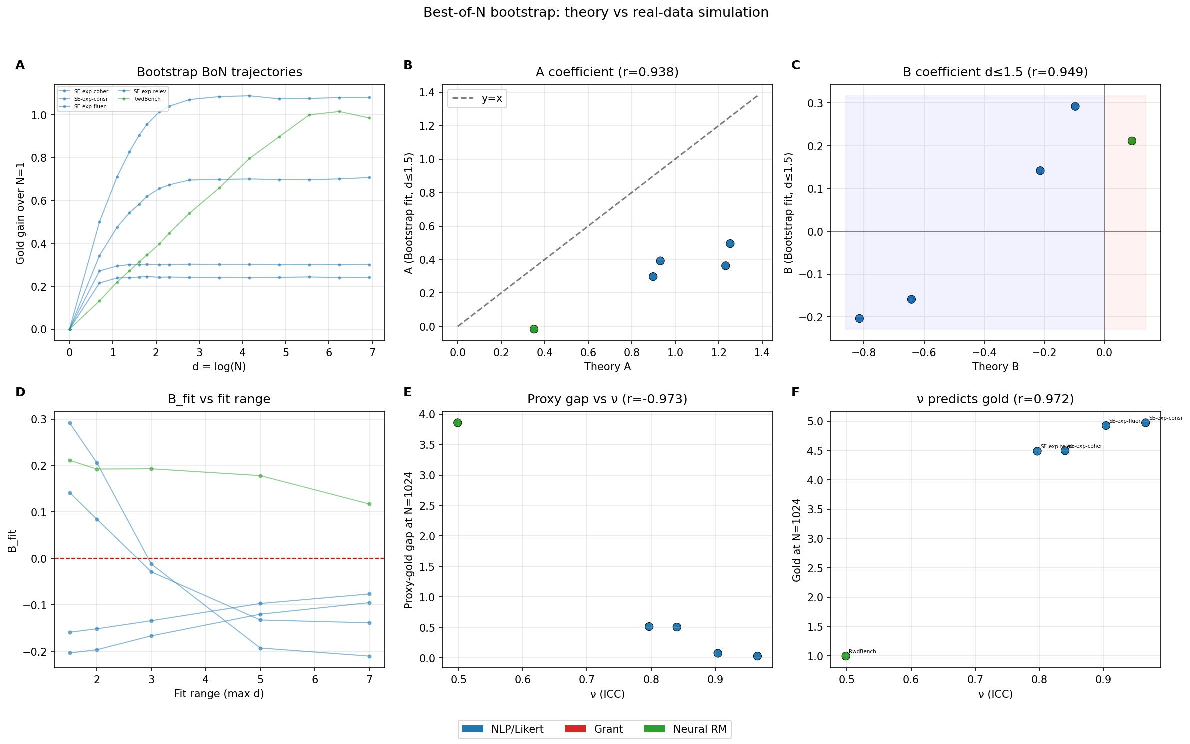
\includegraphics[width=570.96bp,height=357.36bp]{fig_bon_bridge_bootstrap_original.pdf}};
\fill[white] (185,0) rectangle (385,12.7);
\node at (285.48,6.3) {\labelchange{Pooled-item BoN resampling audit}{Best-of-N bootstrap: theory vs real-data simulation}};

% Bridge coordinate, including the fit-window labels in panels B--D.
\fill[white] (65,171.7) rectangle (148,183.5);
\node at (105.35,177.5) {\labelchange{$u=\log N$ (not KL)}{$d=\log(N)$}};
\fill[white] (190.7,68) rectangle (201.7,150);
\node[rotate=90] at (196.2,109) {\labelchange{$A_{\rm fit}$, $u\le1.5$}{A (Bootstrap fit, $d\le1.5$)}};
\fill[white] (373,68) rectangle (383.9,150);
\node[rotate=90] at (378.45,109) {\labelchange{$B_{\rm fit}$, $u\le1.5$}{B (Bootstrap fit, $d\le1.5$)}};
\fill[white] (408,28.4) rectangle (552,40.4);
\node at (480,34.4) {\labelchange{$B$ coefficient, $u\le1.5$ ($r=0.949$)}{$B$ coefficient $d\le1.5$ ($r=0.949$)}};
\fill[white] (64,328.7) rectangle (147,340.4);
\node at (105.35,334.6) {\labelchange{Fit range (max $u$)}{Fit range (max $d$)}};

% nu is SD(gold)/SD(proxy), not an intraclass correlation.
\fill[white] (239,328.7) rectangle (335,340.4);
\node at (287.5,334.6) {\labelchange{$\nu=\sigma_J/\sigma_r$ (SD ratio)}{$\nu$ (ICC)}};
\fill[white] (423,328.7) rectangle (536,340.4);
\node at (479.6,334.6) {\labelchange{$\nu=\sigma_J/\sigma_r$ (SD ratio)}{$\nu$ (ICC)}};

% Panel F is the selected gold level. Panel A already reports a gain.
\fill[white] (375.6,217) rectangle (387.0,301);
\node[rotate=90] at (381.3,259.4) {\labelchange{Gold level at $N=1024$}{Gold at $N=1024$}};
\fill[white] (411,185.5) rectangle (552,197.1);
\node at (480,192) {\labelchange{Gold level vs.\ $\nu$ ($r=0.972$)}{$\nu$ predicts gold ($r=0.972$)}};
\end{tikzpicture}
\end{document}
'
% The original PDF is embedded unchanged. Only label areas are covered.
\documentclass[tikz,border=0pt]{standalone}
\usepackage[OT1]{fontenc}
\usepackage{amsmath,graphicx,xcolor}
\newcommand{\labelchange}[2]{%
  \ifdefined\cleanreview #1\else\textcolor{red}{#1}\\\textcolor{blue}{(#2)}\fi}
\begin{document}
\begin{tikzpicture}[x=1bp,y=-1bp,every node/.style={inner sep=0pt,align=center,font=\sffamily\fontsize{5}{5.5}\selectfont}]
\node[anchor=north west] at (0,0) {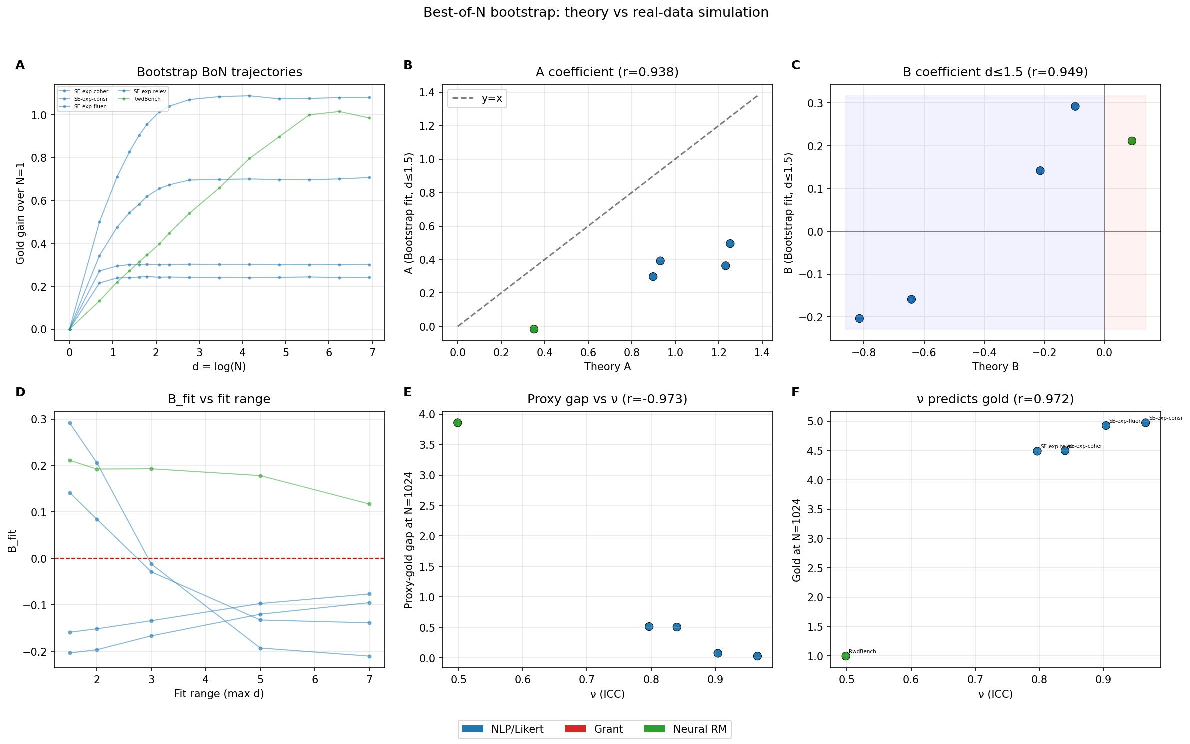
\includegraphics[width=570.96bp,height=357.36bp]{fig_bon_bridge_bootstrap_original.pdf}};
\fill[white] (185,0) rectangle (385,12.7);
\node at (285.48,6.3) {\labelchange{Pooled-item BoN resampling audit}{Best-of-N bootstrap: theory vs real-data simulation}};

% Bridge coordinate, including the fit-window labels in panels B--D.
\fill[white] (65,171.7) rectangle (148,183.5);
\node at (105.35,177.5) {\labelchange{$u=\log N$ (not KL)}{$d=\log(N)$}};
\fill[white] (190.7,68) rectangle (201.7,150);
\node[rotate=90] at (196.2,109) {\labelchange{$A_{\rm fit}$, $u\le1.5$}{A (Bootstrap fit, $d\le1.5$)}};
\fill[white] (373,68) rectangle (383.9,150);
\node[rotate=90] at (378.45,109) {\labelchange{$B_{\rm fit}$, $u\le1.5$}{B (Bootstrap fit, $d\le1.5$)}};
\fill[white] (408,28.4) rectangle (552,40.4);
\node at (480,34.4) {\labelchange{$B$ coefficient, $u\le1.5$ ($r=0.949$)}{$B$ coefficient $d\le1.5$ ($r=0.949$)}};
\fill[white] (64,328.7) rectangle (147,340.4);
\node at (105.35,334.6) {\labelchange{Fit range (max $u$)}{Fit range (max $d$)}};

% nu is SD(gold)/SD(proxy), not an intraclass correlation.
\fill[white] (239,328.7) rectangle (335,340.4);
\node at (287.5,334.6) {\labelchange{$\nu=\sigma_J/\sigma_r$ (SD ratio)}{$\nu$ (ICC)}};
\fill[white] (423,328.7) rectangle (536,340.4);
\node at (479.6,334.6) {\labelchange{$\nu=\sigma_J/\sigma_r$ (SD ratio)}{$\nu$ (ICC)}};

% Panel F is the selected gold level. Panel A already reports a gain.
\fill[white] (375.6,217) rectangle (387.0,301);
\node[rotate=90] at (381.3,259.4) {\labelchange{Gold level at $N=1024$}{Gold at $N=1024$}};
\fill[white] (411,185.5) rectangle (552,197.1);
\node at (480,192) {\labelchange{Gold level vs.\ $\nu$ ($r=0.972$)}{$\nu$ predicts gold ($r=0.972$)}};
\end{tikzpicture}
\end{document}
'
% The original PDF is embedded unchanged. Only label areas are covered.
\documentclass[tikz,border=0pt]{standalone}
\usepackage[OT1]{fontenc}
\usepackage{amsmath,graphicx,xcolor}
\newcommand{\labelchange}[2]{%
  \ifdefined\cleanreview #1\else\textcolor{red}{#1}\\\textcolor{blue}{(#2)}\fi}
\begin{document}
\begin{tikzpicture}[x=1bp,y=-1bp,every node/.style={inner sep=0pt,align=center,font=\sffamily\fontsize{5}{5.5}\selectfont}]
\node[anchor=north west] at (0,0) {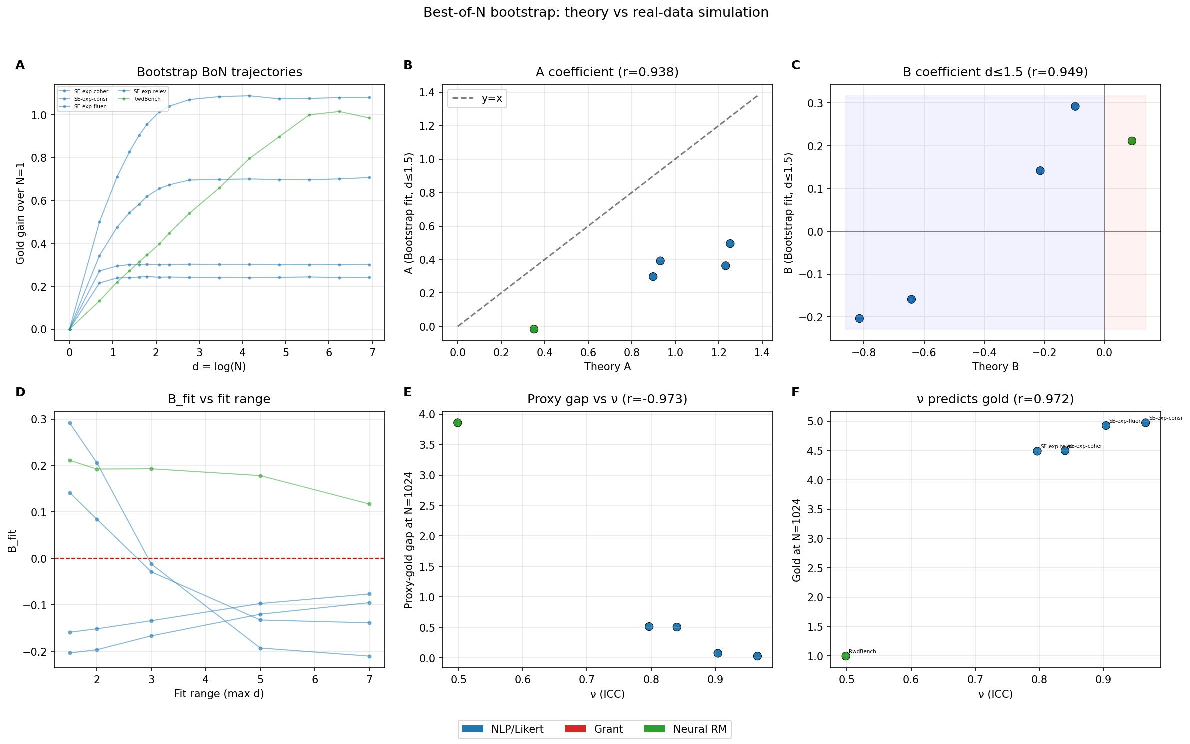
\includegraphics[width=570.96bp,height=357.36bp]{fig_bon_bridge_bootstrap_original.pdf}};
\fill[white] (185,0) rectangle (385,12.7);
\node at (285.48,6.3) {\labelchange{Pooled-item BoN resampling audit}{Best-of-N bootstrap: theory vs real-data simulation}};

% Bridge coordinate, including the fit-window labels in panels B--D.
\fill[white] (65,171.7) rectangle (148,183.5);
\node at (105.35,177.5) {\labelchange{$u=\log N$ (not KL)}{$d=\log(N)$}};
\fill[white] (190.7,68) rectangle (201.7,150);
\node[rotate=90] at (196.2,109) {\labelchange{$A_{\rm fit}$, $u\le1.5$}{A (Bootstrap fit, $d\le1.5$)}};
\fill[white] (373,68) rectangle (383.9,150);
\node[rotate=90] at (378.45,109) {\labelchange{$B_{\rm fit}$, $u\le1.5$}{B (Bootstrap fit, $d\le1.5$)}};
\fill[white] (408,28.4) rectangle (552,40.4);
\node at (480,34.4) {\labelchange{$B$ coefficient, $u\le1.5$ ($r=0.949$)}{$B$ coefficient $d\le1.5$ ($r=0.949$)}};
\fill[white] (64,328.7) rectangle (147,340.4);
\node at (105.35,334.6) {\labelchange{Fit range (max $u$)}{Fit range (max $d$)}};

% nu is SD(gold)/SD(proxy), not an intraclass correlation.
\fill[white] (239,328.7) rectangle (335,340.4);
\node at (287.5,334.6) {\labelchange{$\nu=\sigma_J/\sigma_r$ (SD ratio)}{$\nu$ (ICC)}};
\fill[white] (423,328.7) rectangle (536,340.4);
\node at (479.6,334.6) {\labelchange{$\nu=\sigma_J/\sigma_r$ (SD ratio)}{$\nu$ (ICC)}};

% Panel F is the selected gold level. Panel A already reports a gain.
\fill[white] (375.6,217) rectangle (387.0,301);
\node[rotate=90] at (381.3,259.4) {\labelchange{Gold level at $N=1024$}{Gold at $N=1024$}};
\fill[white] (411,185.5) rectangle (552,197.1);
\node at (480,192) {\labelchange{Gold level vs.\ $\nu$ ($r=0.972$)}{$\nu$ predicts gold ($r=0.972$)}};
\end{tikzpicture}
\end{document}
'
% The original PDF is embedded unchanged. Only label areas are covered.
\documentclass[tikz,border=0pt]{standalone}
\usepackage[OT1]{fontenc}
\usepackage{amsmath,graphicx,xcolor}
\newcommand{\labelchange}[2]{%
  \ifdefined\cleanreview #1\else\textcolor{red}{#1}\\\textcolor{blue}{(#2)}\fi}
\begin{document}
\begin{tikzpicture}[x=1bp,y=-1bp,every node/.style={inner sep=0pt,align=center,font=\sffamily\fontsize{5}{5.5}\selectfont}]
\node[anchor=north west] at (0,0) {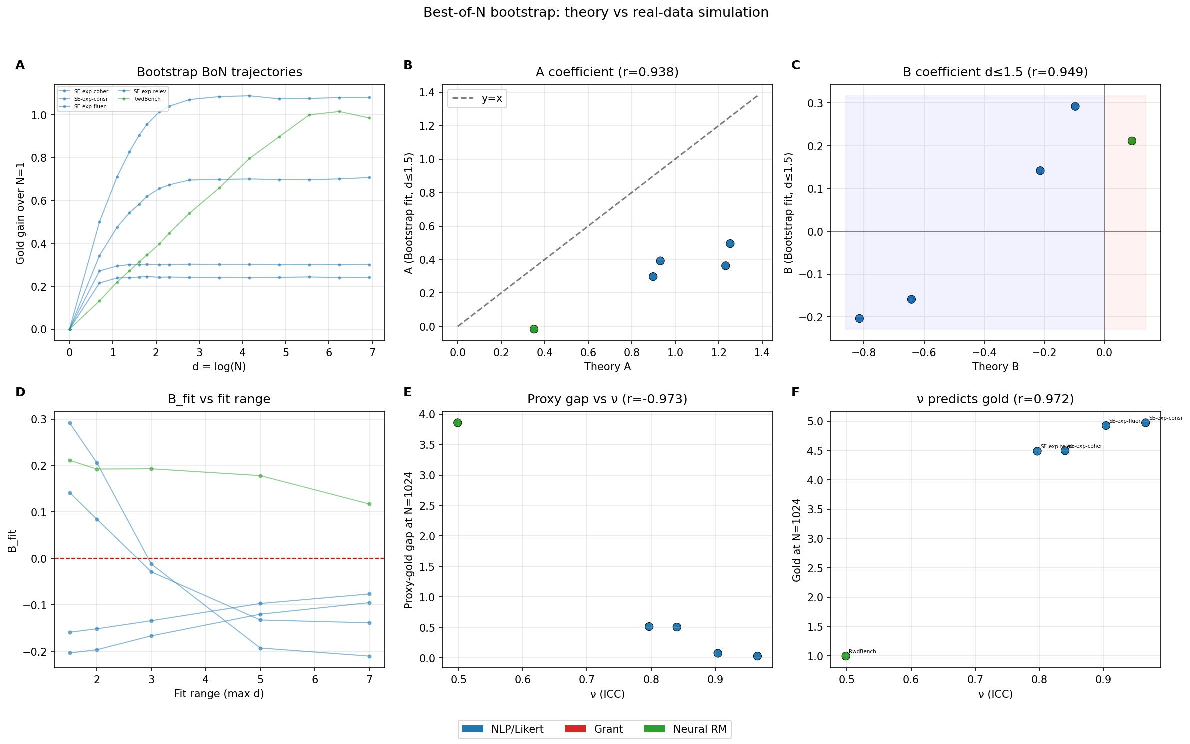
\includegraphics[width=570.96bp,height=357.36bp]{fig_bon_bridge_bootstrap_original.pdf}};
\fill[white] (185,0) rectangle (385,12.7);
\node at (285.48,6.3) {\labelchange{Pooled-item BoN resampling audit}{Best-of-N bootstrap: theory vs real-data simulation}};

% Bridge coordinate, including the fit-window labels in panels B--D.
\fill[white] (65,171.7) rectangle (148,183.5);
\node at (105.35,177.5) {\labelchange{$u=\log N$ (not KL)}{$d=\log(N)$}};
\fill[white] (190.7,68) rectangle (201.7,150);
\node[rotate=90] at (196.2,109) {\labelchange{$A_{\rm fit}$, $u\le1.5$}{A (Bootstrap fit, $d\le1.5$)}};
\fill[white] (373,68) rectangle (383.9,150);
\node[rotate=90] at (378.45,109) {\labelchange{$B_{\rm fit}$, $u\le1.5$}{B (Bootstrap fit, $d\le1.5$)}};
\fill[white] (408,28.4) rectangle (552,40.4);
\node at (480,34.4) {\labelchange{$B$ coefficient, $u\le1.5$ ($r=0.949$)}{$B$ coefficient $d\le1.5$ ($r=0.949$)}};
\fill[white] (64,328.7) rectangle (147,340.4);
\node at (105.35,334.6) {\labelchange{Fit range (max $u$)}{Fit range (max $d$)}};

% nu is SD(gold)/SD(proxy), not an intraclass correlation.
\fill[white] (239,328.7) rectangle (335,340.4);
\node at (287.5,334.6) {\labelchange{$\nu=\sigma_J/\sigma_r$ (SD ratio)}{$\nu$ (ICC)}};
\fill[white] (423,328.7) rectangle (536,340.4);
\node at (479.6,334.6) {\labelchange{$\nu=\sigma_J/\sigma_r$ (SD ratio)}{$\nu$ (ICC)}};

% Panel F is the selected gold level. Panel A already reports a gain.
\fill[white] (375.6,217) rectangle (387.0,301);
\node[rotate=90] at (381.3,259.4) {\labelchange{Gold level at $N=1024$}{Gold at $N=1024$}};
\fill[white] (411,185.5) rectangle (552,197.1);
\node at (480,192) {\labelchange{Gold level vs.\ $\nu$ ($r=0.972$)}{$\nu$ predicts gold ($r=0.972$)}};
\end{tikzpicture}
\end{document}
